%!TEX root = ./main.tex

\section[The question]{The Question}

% SECTION TIMING: 0:00--8:00 (3 frames).
% LAYOUT RULES: frame title on one line (< ~44 chars); one figure per frame; the
% figure is the slide -- the words below it are what you say, not what they read.
% RUNNING EXAMPLE (used from Section 3 on): 5 GHz Wi-Fi, lambda = 6 cm, antennas
% lambda/2 apart; phone at 30 degrees -> each next antenna lags a QUARTER TURN.

% Teaching note (150 s): start with the want, not the technique. Walk the photos:
% a museum map on your phone, VR, a delivery drone. All of them need "where am I"
% INDOORS. Ask who has used Google Maps inside a mall, and how well it went.
\begin{frame}{Where is the phone?}
  \vspace{0.2em}
  \centering
  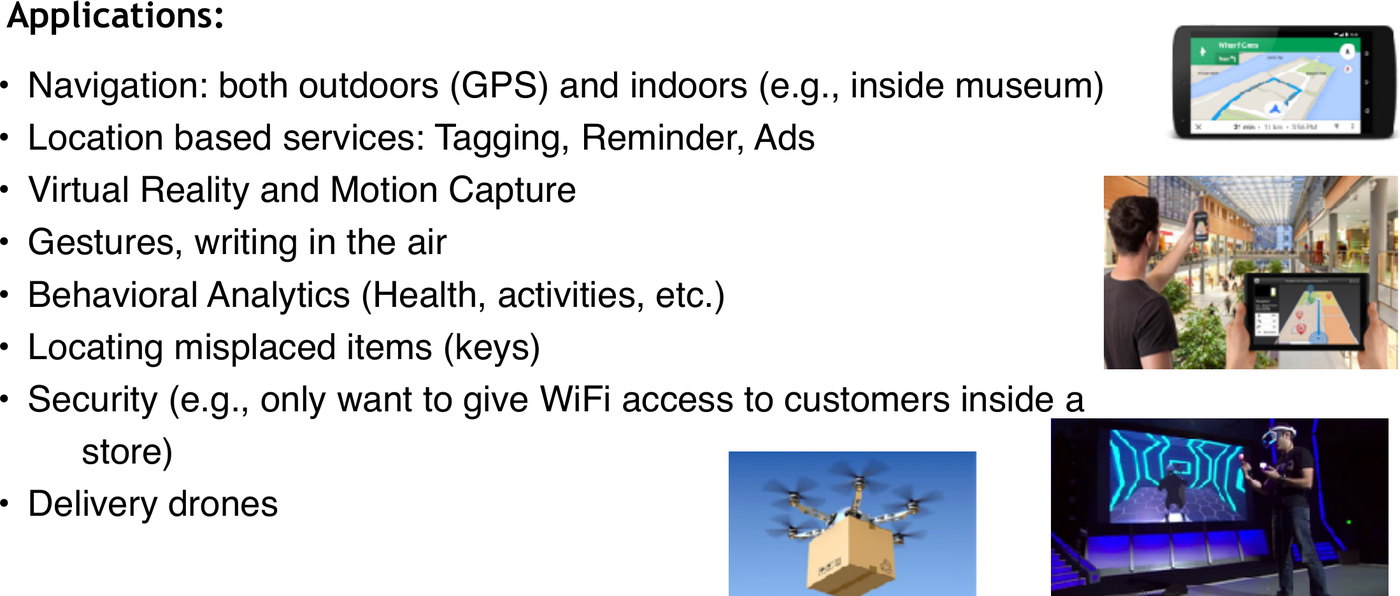
\includegraphics[width=0.9\textwidth]{figure/mit_applications.png}

  \vspace{0.4em}
  \takeaway{Every one of these needs a position --- \textbf{indoors},\\
    where the one positioning system everybody knows does not reach.}
  \source{https://www.mit.edu/~fadel/courses/MAS.s60/materials/Lec2-localization-2022.pdf}{Figure: Adib \& Eid, MIT MAS.S60 Lecture 2, ``Fundamentals of Wireless Sensing \& Localization''}
\end{frame}

% Teaching note (120 s): GPS = meters, outdoors only; indoors it fades. Point at
% the red lines: known indoor options are either not accurate (Wi-Fi RSSI) or need
% new hardware (ultrasound) or cameras. Then the observation the lecture rides on.
\begin{frame}{Outdoors: GPS. Indoors: nothing good}
  \vspace{0.2em}
  \centering
  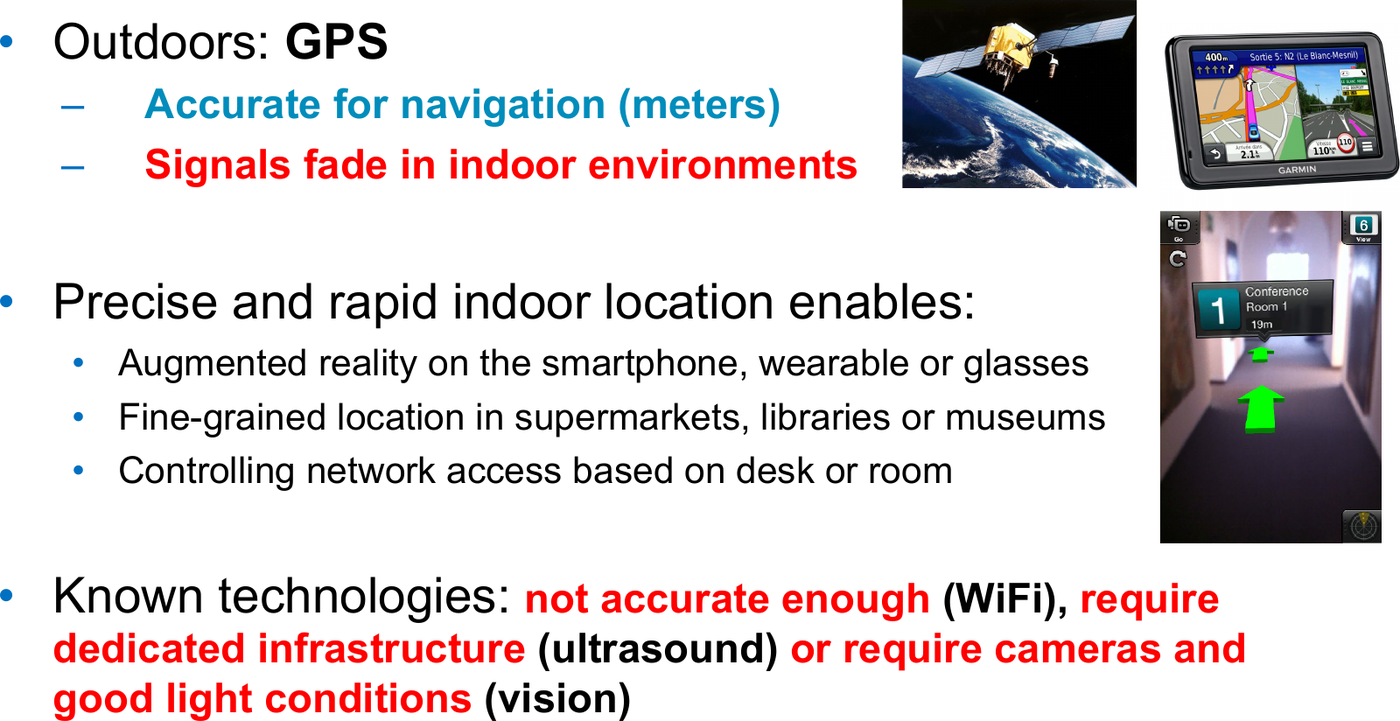
\includegraphics[width=0.86\textwidth]{figure/at_why_indoor.png}

  \vspace{0.4em}
  \ask{Every building already has Wi-Fi.\\
    Can the access point itself work out where the phone is?}
  \source{https://www.usenix.org/conference/nsdi13/technical-sessions/presentation/xiong}{Figure: Xiong \& Jamieson, ArrayTrack talk, NSDI 2013}
\end{frame}

% Teaching note (150 s): two ways to run localization. GPS: the DEVICE listens to
% anchors. Radar / Wi-Fi: the NETWORK listens to the device. Today is the second
% kind -- the AP hears the phone's packet anyway. What can it measure from that
% packet? Announce the ladder: power -> phase -> angle -> distance.
\begin{frame}{Who does the locating?}
  \vspace{0.2em}
  \centering
  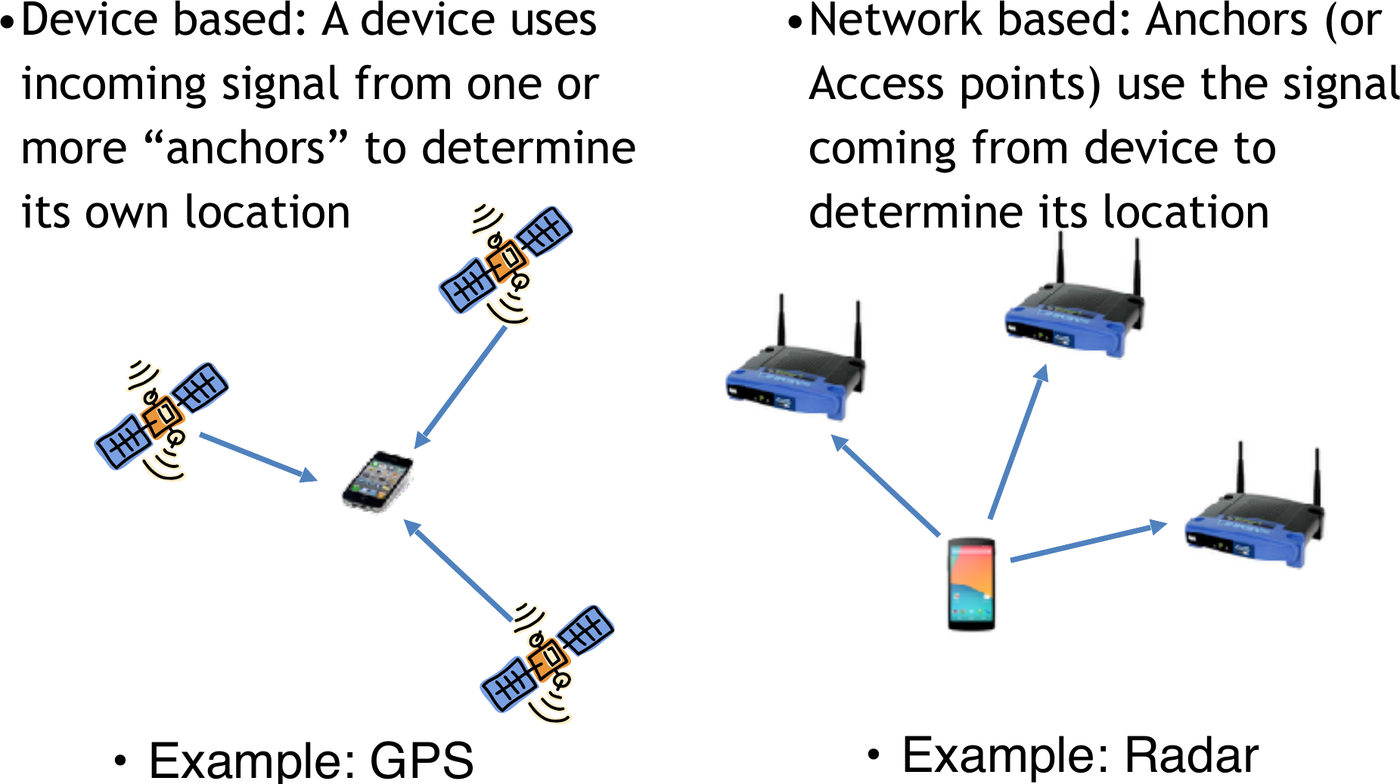
\includegraphics[width=0.9\textwidth]{figure/mit_who_localizes.png}

  \vspace{0.4em}
  {\small Today: \textbf{network-based}. The AP hears the phone's packet anyway.
   What can it measure from it?\par}
  \vspace{0.3em}
  {\small\centering
    \textcolor{softgray}{signal strength} $\;\to\;$
    \textcolor{ranblue}{phase} $\;\to\;$
    \textcolor{ranblue}{\textbf{angle}} $\;\to\;$
    \textcolor{coreorange}{\textbf{distance}} $\;\to\;$
    \textcolor{softgreen}{\textbf{both}}\par}
  \source{https://www.mit.edu/~fadel/courses/MAS.s60/materials/Lec2-localization-2022.pdf}{Figure: MIT MAS.S60 Lecture 2}
\end{frame}
